\chapter{Methodology} \label{chap:methodolo}

\section{Datasets}

Selecting appropriate datasets is pivotal in the development, training, and evaluation of recognition models. In this study, we employ three widely recognized datasets: the Ryerson Audio-Visual Database of Emotional Speech and Song (RAVDESS), the Berlin Database of Emotional Speech (Emo-DB), and the Human Activity Recognition Using Smartphones (HAR) dataset. While RAVDESS and Emo-DB are commonly used in speech emotion classification—featuring emotionally expressive performances by professional actors in a UTS—the HAR dataset represents a MTS dataset collected from wearable sensors for activity recognition. The following subsections provide detailed descriptions of each dataset, highlighting their key features, structures, and the rationale for their use in this study.

\subsection{Ryerson Audio-Visual Database of Emotional Speech and Song} % https://zenodo.org/records/1188976#.YFZuJ0j7SL8

The Ryerson Audio-Visual Database of Emotional Speech and Song (RAVDESS) \cite{ravdess} is a widely recognized benchmark dataset utilized extensively in audiovisual emotion classification research \cite{anusha2021, vimal2021, abdullah2020}. The dataset consists of short audio and video recordings that feature both spoken and sung performances, enacted by a cohort of 24 actors (12 male and 12 female). Each recording is labeled with one of the following emotion categories: \textit{angry}, \textit{calm}, \textit{disgust}, \textit{fearful}, \textit{happy}, \textit{neutral}, \textit{sad}, and \textit{surprised}.

To promote consistency and reproducibility, each actor delivers two predefined phrases in English: ``Kids are talking by the door'' and ``Dogs are sitting by the door.'' Apart from the neutral category, all emotions are expressed at two distinct intensity levels (normal and strong), with each instance repeated twice. These structured variations in emotional intensity, repetition, and diversity of vocal expressions make RAVDESS an invaluable asset for the development and validation of emotion recognition models in a wide range of applications.

For the audio-only subset of the dataset which we employ for further analysis in the present work, there are a total of $1440$ speech recordings and $1012$ song recordings. It is worth noting that the singing subset is slightly smaller, as one actor's data is missing, and the emotions \textit{sad} and \textit{surprised} are not included for singing performances.

Despite its favorable reception within the academic community, as demonstrated by its widespread adoption, evidence suggests that the application of RAVDESS in real-world scenarios may lead to underwhelming results \cite{churaev2021}. One possible explanation for this discrepancy is the issue of data leakage. Specifically, an overlap of similar samples between the training and validation sets may result in unintended information sharing, thereby artificially inflating performance metrics. This overestimation does not accurately reflect the generalizability and practical effectiveness of models when deployed in real-world environments.

\subsection{Berlin Database of Emotional Speech} % http://www.emodb.bilderbar.info/download/

The Berlin Database of Emotional Speech (Emo-DB) \cite{emodb}, akin to RAVDESS, is a well-regarded dataset for speech emotion classification tasks \cite{sinith2015, kotti2008, ying2010}. It comprises short spoken audio recordings performed by 10 professional actors (5 male and 5 female), each enacting various grammatical phrases in German, as detailed in Table~\ref{tab:emodb}. Each recording is annotated with one of the following emotion categories: \textit{anger}, \textit{anxiety/fear}, \textit{boredom}, \textit{disgust}, \textit{happiness}, \textit{neutral}, and \textit{sadness}.

To ensure the quality and reliability of the dataset, these samples underwent evaluation by a significant number of listeners, who assessed the naturalness of the emotional expressions. In total, the dataset comprises $535$ speech files.

\begin{center}
    \begin{longtable}{*{2}{p{.45\linewidth}}}
        \caption{Grammatical phrases in the Emo-DB dataset\label{tab:emodb}}                                                                                         \\
        \specialrule{1.5pt}{2pt}{2pt}
        German                                                                             & English                                                                 \\
        \specialrule{0.3pt}{2pt}{2pt}
        \endfirsthead

        \specialrule{1.5pt}{2pt}{2pt}
        German                                                                             & English                                                                 \\
        \specialrule{0.3pt}{2pt}{2pt}
        \endhead

        \specialrule{0.3pt}{2pt}{2pt}
        \multicolumn{2}{c}{{Continued on the next page}}                                                                                                             \\
        \specialrule{0.3pt}{2pt}{2pt}
        \endfoot
        \endlastfoot

        Der Lappen liegt auf dem Eisschrank.                                               & The cloth is on the refrigerator.                                       \\
        Das will sie am Mittwoch abgeben.                                                  & She will deliver it on Wednesday.                                       \\
        Heute abend könnte ich es ihm sagen.                                               & Tonight I could tell him.                                               \\
        Das schwarze Stück Papier befindet sich da oben neben dem Holzstück.               & The black sheet of paper is located up there next to the piece of wood. \\
        In sieben Stunden wird es soweit sein.                                             & In seven hours it will be time.                                         \\
        Was sind denn das für Tüten, die da unter dem Tisch stehen?                        & What about the bags that are under the table?                           \\
        Sie haben es gerade hochgetragen und jetzt gehen sie wieder runter.                & They just carried it upstairs and now they are going back down.         \\
        An den Wochenenden bin ich jetzt immer nach Hause gefahren und habe Agnes besucht. & On weekends, I now always went home and visited Agnes.                  \\
        Ich will das eben wegbringen und dann mit Karl was trinken gehen.                  & I will just take this away and then go have a drink with Karl.          \\
        Die wird auf dem Platz sein, wo wir sie immer hinlegen.                            & It will be in the place where we always put it.                         \\
        \specialrule{1.5pt}{2pt}{2pt}
    \end{longtable}
    Source: Own authorship
\end{center}

\subsection{Human Activity Recognition Using Smartphones}

The Human Activity Recognition Using Smartphones (HAR) dataset~ \cite{ortiz2013} represents a distinct category of data compared to the speech-focused RAVDESS and Emo-DB datasets. While the latter are centered around audio signals for emotion recognition, the HAR dataset consists of MTS data collected from wearable sensors, specifically accelerometers and gyroscopes embedded in smartphones. This fundamental difference not only sets it apart in terms of data modality but also introduces unique challenges and considerations in the modeling process.

The dataset was constructed using data from $30$ volunteers aged between $19$ and $48$ years. Each participant performed six predefined physical activities while carrying a waist-mounted Samsung Galaxy S $\text{II}$ smartphone. The activities included: \textit{walking}, \textit{walking upstairs}, \textit{walking downstairs}, \textit{sitting}, \textit{standing}, and \textit{laying}.

Sensor signals were recorded at a constant sampling rate of $50\,\text{ Hz}$, capturing $3$-axial linear acceleration and 3-axial angular velocity. The raw sensor data underwent preprocessing steps, including noise filtering and normalization. Subsequently, the data were segmented into fixed-width sliding windows of $2.56$ seconds (equivalent to $128$ readings per window) with a $50\%$ overlap between consecutive windows. This segmentation resulted in a rich set of time series samples that capture the dynamic patterns associated with each physical activity.

The MTS nature of the HAR dataset introduces complexities not present in UTS data like audio signals. Modeling such data requires capturing not only temporal dependencies but also the interrelationships between different sensor modalities. This necessitates advanced techniques capable of handling high-dimensional inputs and learning intricate patterns across multiple variables.

In this study, the HAR dataset serves as a means to evaluate the adaptability and robustness of the NVAR kernel when applied to MTS data. For consistency and to focus on the raw data's representational capacity, we utilize the HAR dataset without additional feature engineering.

\section{Data Preprocessing}

Preprocessing is a critical step to ensure that the audio data from the RAVDESS and Emo-DB datasets are in a suitable format for analysis and modeling. The preprocessing pipeline was implemented using the \texttt{librosa} library in Python \cite{librosa}, and it consisted of the following steps:

\subsection{Audio Loading and Resampling}

All audio files were loaded in mono format at a standardized sampling rate of $8\,\text{kHz}$ using the \texttt{librosa.load} function and cropped to a maximum duration of $3$ seconds. This resampling helps to reduce computational complexity and ensures consistency across all audio samples.

\begin{figure}[H]
  \centering
  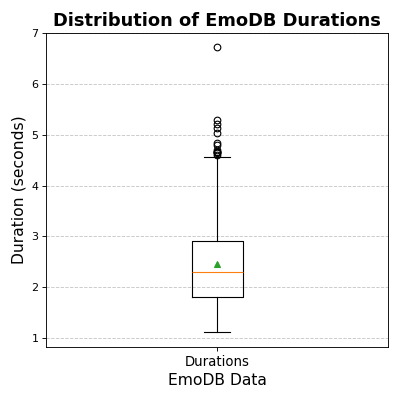
\includegraphics[width = 2.5in, keepaspectratio]{figures/Durations Box Plot - EmoDB.png}
  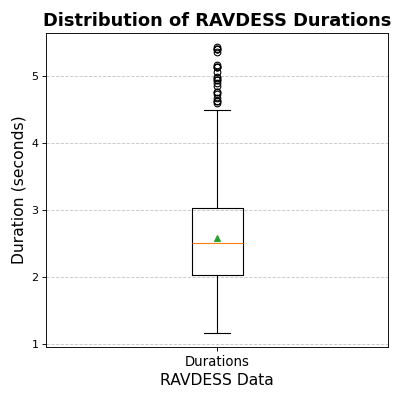
\includegraphics[width = 2.5in, keepaspectratio]{figures/Durations Box Plot - RAVDESS.png}
  \caption{Durations Box Plot}
\end{figure}

\subsection{Vocal Separation}

To isolate the vocal components and reduce background noise, an adaptive filtering technique was applied. This process began with computing the short-time Fourier transform (STFT) of the audio signal to obtain its magnitude and phase components. Non-negative matrix factorization (NMF) filtering was then used to separate the vocal content from other elements. A soft mask was subsequently applied to enhance the separation between vocal and non-vocal elements, and, finally, the time-domain signal was reconstructed using the inverse STFT.

\subsection{Silence Removal}

To focus on the significant parts of the speech and eliminate silence or low-ampli\-tude sections, the audio signals were trimmed based on an amplitude threshold. This was done using the \texttt{librosa.effects.split} function, which identifies intervals where the signal is above a certain decibel level (\texttt{top\_db} parameter). The segments were then concatenated to form the final processed signal.

\subsection{Padding and Alignment}

For samples shorter than the desired duration, zero-padding was applied to align all audio samples to a uniform length. This ensures that the input data has consistent dimensions, which is essential for batch processing in machine learning models.

\subsection{Final Preprocessing Pipeline}

The entire preprocessing routine was encapsulated in a function that loads the audio file, applies vocal separation, removes silence, and pads the signal as needed.

\section{Evaluation Method and Metrics}

We employed the proposed NVAR kernel for classifying both UTS and MTS, using a Support Vector Machine (SVM) classifier with 10-fold cross-validation to fine-tune the hyperparameter $C$. The performance was evaluated using either accuracy or weighted F1-score as the scoring metric for cross-validation. Each classification experiment was repeated over 10 iterations per dataset, with the cross-validation data split randomized in each iteration to ensure robustness. This evaluation pipeline, as suggested by the original authors, was applied to our selected UTS datasets (RAVDESS and Emo-DB) and the MTS dataset (HAR). All experiments were conducted in our personal computers with limited hardware. 

To assess classification performance on both training and testing sets, we computed accuracy, weighted precision, weighted recall, and weighted F1-score. These metrics allowed us to account for class imbalances within the datasets, ensuring a balanced evaluation across all classes. Accuracy was included to facilitate comparisons with existing methods in the literature, while precision, recall, and F1-score provided a comprehensive view of the classifier’s effectiveness across imbalanced classes. Additionally, we record the total running time for training and testing each dataset to evaluate the computational efficiency of the proposed method.

To further examine the impact of class imbalance on classification performance, we computed the confusion matrix and analyzed the class distribution for the testing sets. This analysis helped identify any biases arising from imbalanced datasets and provided insights into the classifier’s strengths and weaknesses in distinguishing between classes.
